%\documentclass[journal]{IEEEtran}
%\documentclass[11pt, a4paper, oneside]{article}
\documentclass[11pt, a4paper, oneside]{article}

\usepackage{appendix}

% Incluimos el paquete Babel que sirve para separar correctamente las palabras de multitud de idiomas.
\usepackage[english]{babel}

% Este paquete permite poner acentos directamente.
%:
\usepackage[latin1]{inputenc}

\usepackage[T1]{fontenc}

\usepackage{comment}

% Macros AMS para teoremas.
\usepackage{amsmath}

% Romper autom·ticamente ecuaciones muy largas
%\usepackage{breqn}

% Permite usar fuentes AMS.
\usepackage{amsfonts}

% Para usar sÌmbolos AMS.
\usepackage{amssymb}



% ?
\usepackage{color}
\definecolor{gray}{rgb}{0.4,0.4,0.4}
\definecolor{darkblue}{rgb}{0.0,0.0,0.6}
\definecolor{cyan}{rgb}{0.0,0.6,0.6}

% Color en las tablas.
\usepackage{colortbl}

% Para usar el símbolo del euro.
\usepackage{eurosym}

%?
\usepackage{listings}

% ?
\usepackage{mathrsfs}

% Uso desconocido.
\usepackage{shadow}

% Espaciado de primera lÌnea de cada p·rrafo.
\usepackage{indentfirst}

% ?
\usepackage{theorem}

% ?
\usepackage{shadow}

% Permite un manejo sencillo de los apÈndices. Permite tambiÈn introducir subapendices.
%\usepackage{appendix} 

%?
\usepackage[pdftex]{graphicx}

% De esta forma aparecen hiperv�culos en el PDF.
\usepackage[colorlinks=true]{hyperref}

% Soporte para el comando \marginsize.
\usepackage{anysize} 

%Permite manejar los m·rgenes de forma sencilla.
\marginsize{3cm}{2cm}{2.5cm}{2.5cm}

\usepackage{url}

% Usado junto con \begin{figure}[H] ... pone la figura exactamente donde yo quiero.
\usepackage{float}

\usepackage[mediumspace,mediumqspace,squaren,binary]{SIunits}
%\sisetup{per-mode=symbol,per-symbol = p}
%\usepackage{siunitx}
%\sisetup{per-mode=symbol,detect-all}
%\usepackage{xfrac}
%\sisetup{per-mode=fraction,fraction-function=\sfrac,alsoload=binary}

%?
\usepackage{subfigure}

%?
\usepackage{verbatim}

% Permite usar el sÌmbolo de euro.
%\usepackage{eurofont}

% ?
%\addtolength{\footskip}{+3cm}

% Para un encabezado especial m·s visual usar
%\usepackage{fancyhdr} y \pagestyle{fancy}             

% Para que el nombre del capitulo salga m·s chulo.
\usepackage[Lenny]{fncychap}
\usepackage{fancyvrb}


% ?
\usepackage{extramarks}

% Para poder intercalar imagen y texto.
\usepackage{wrapfig} 
\usepackage{multicol}
\usepackage{rotating}
\setlength\unitlength{1mm}

\linespread{1.5}

% Declare the extension of the images you are going to use, so you won't have to specify these with
% every instance of \includegraphics
\DeclareGraphicsExtensions{.jpg, .pdf, .mps, .png, .gif, .fig, .bmp, .svg}

\setlength\parindent{0pt}

\title{\textbf{The pure pursuit path following algorithm}}
\author{Juan Francisco Rasc\'on Crespo\\
    juan.rascon@eurecat.org}
\date{}

\begin{document}

\maketitle

\section{Introduction}

This document is just a summary of some documents I have worked with when developing the pure pursuit algorithm for a project in the company I work for, Eurecat. Given the general success of this algorithm in literature and its simplicity, it is likely that it will be used again in forthcoming land-based-navigation projects, so I decided to compile here my notes for future reference.

This document aims to expose the geometric derivation for the path following algorithm called pure pursuit for differential drives.

This report also includes a geometric derivation of the method, and presents some insights into the performance of the algorithm as a function of its parameters.\\

The pure pursuit algorithm is a tracking algorithm that works by calculating the \textbf{curvature}, $\gamma$, that will move a vehicle \textbf{from its current position to some chosen path position}. The whole point of the algorithm is to choose a goal position that is \textbf{some distance ahead of the vehicle on the path} (a waypoint). The name pure pursuit comes from the analogy that it is used to describe the method. \textit{We tend to think of the vehicle as chasing a point on the path some distance ahead of it, i.e., it is pursuing that moving point}. That analogy is often used to compare this method to \textit{the way humans drive}. We tend to look some distance in front of the car and head toward that spot. This lookahead distance, denoted as $L_{ah}$, changes as we drive to reflect the twist of the road and vision occlusions.

\section{Geometric derivation}

The pure pursuit algorithm is a method of geometrically determining the curvature that will drive the vehicle to a goal point. This goal point is a point on the path that is one lookahead distance, $L_{ah}$, from the current vehicle's position. An arc that joins the current vehicle's position and the goal point is found out. The chord of this arc is the lookahead distance, and this is a constraint in determining the unique arc that joins the two points. Consider the lookahead distance to be analogous to the distance to a spot in front of a car that a human driver might look toward to track the roadway. The result of the algorithm is the curvature, $\gamma$ of the arc that joins the vehicle's position to the chosen goal point and whose chord length is $L_{ah}$

\begin{figure}[H]
  \begin{center}
    \includegraphics[scale=0.85]{Images/pure_pursuit_img.pdf}
    \caption{Geometric analysis for the pure pursuit algorithm.}
    \label{fig:Pure_pursuit}
  \end{center}
\end{figure}

\begin{align}
L_{ah}&\,=\,\sqrt{\left(x_{g}\,-\,x_r\right)^2\,+\,\left(y_{g}\,-\,y_r\right)^2}\\
&\,=\,\sqrt{{x_{g}^*}^2\,+\,{y_{g}^*}^2}
\end{align}

\begin{align}
\theta_{err}&\,=\,\alpha\,-\,\theta_r\\
\,&=\,\arctan\left(\frac{y_{g}\,-\,y_r}{x_{g}\,-\,x_r}\right)\,-\,\theta_r
\end{align} 

\begin{align}
R&\,=\,d\,+\,y_{g}^*\\
R^2&\,=\,d^2\,+\,{x_g^*}^2\\
&\,=\,\left(R\,-\,y_g^*\right)^2\,+\,{x_g^*}^2
\label{Eq:pp1}
\end{align}

\begin{align}
R^2&\,=\,R^2\,-\,2\,R\,y_g^*\,+\,{y_g^*}^2\,+\,{x_g^*}^2
\label{Eq:pp2}
\end{align}

Since 

\begin{align}
L_{ah}\,&=\,\sqrt{{x_{g}^*}^2\,+\,{y_{g}^*}^2}\\ y_g^*\,&=\,L_{ah}\,\sin\left(\theta_{err}\right)\\
\label{Eq:pp3}
\end{align}

equation \ref{Eq:pp2} becomes:

\begin{align}
L_{ah}^2&\,=\,2\,R\,y_g^*\\
\,&=\,2\,R\,L_{ah}\,\sin\left(\theta_{err}\right)\\
L_{ah}\,&=\,2\,R\,\sin\left(\theta_{err}\right)
\label{Eq:pp4}
\end{align}

Finally:
\begin{align}
\gamma\,=\,\frac{1}{R}\,=\,\frac{2\,\sin\left(\theta_{err}\right)}{L_{ah}}
\label{Eq:pp5}
\end{align}

\section{Implementation}

The implementation of the pure pursuit algorithm is fairly straightforward. The pure pursuit algorithm can be outlined as follows:

\begin{itemize}
  \item Determine the robot's current location.
  \item Find the path's goal waypoint to navigate to. This action can be done in different ways. The way I have implemented this now is that in the software I store the path's index for the last goal waypoint the robot navigated to because this waypoint was one lookahead distance from it. Next time the algorithm has to find a goal point that is one lookahead distance from the robot's position, it starts looking from this index onwards, selecting the first waypoint that satisfies this distance constraint.
  \item Calculate the curvature using the previous equations and request the vehicle to set the steering to that curvature.
  \item Back to the first step.
\end{itemize}

\section{Effects of changing the lookahead distance}

There is one parameter in the pure pursuit algorithm, the lookahead distance.
The effects of changing the parameter $L_{ah}$ are easy to imagine using the analogy to human driving.

\begin{figure}[H]
    \begin{center}
        \includegraphics[scale=0.76]{Images/lookahead_distance_effect.png}
        \caption{Effect of $L_{ah}$ in the tracking behaviour.}
        \label{fig:lookahead_distance_effect}
    \end{center}
\end{figure}

\textbf{Longer lookahead distances tend to converge to the path more gradually and with less oscillation}. The response of the pure pursuit tracker looks similar to the step response of a second-order dynamic system and the value of $L_{ah}$ tends to act as a damping factor.

\textbf{The longer the lookahead distance, the less \textit{curvy} of a path that can be followed}. The algorithm is calculating a curvature so that the vehicle can drive an arc. If the path between the vehicle and the goal point is sufficiently \textit{curvy} then there might not be an arc that uses the current value of $L_{ah}$ to join the two points; any driven arc will induce error.

Just a final word about the lookahead distance. Try to make it at least equal to the differential base's track width (distance between wheels). That way, in the unusual case when $\theta_{err}\,=\,\frac{\pi}{2}$, the radius $R$ is half the distance between wheels and in that case the robot will turn around one of the wheels, while the other will remain stopped. If the lookahead distance is less than the track width, then in the weird case when $\theta_{err}\,=\,\frac{\pi}{2}$ the turning radius, $R$, will be less than half the distance between wheels and then the robot will turn around a point that is located somewhere in between one of the wheels and the robot's center, and even when this is not harmful it is not very useful.
 
A video showing this: \url{https://tinyurl.com/y6ox5zee}


\section{How to command the differential drive to follow the curvature}

Since we are commanding a differential drive, we have to tell the low-level controller the linear speed, $v$, and the angular speed, $\omega$, for the robot to achieve the desired curvature.
The pure pursuit algorithm does not tell you what values are for these speeds; therefore, here you have to be creative and design a strategy that fits your application and your platform. I'll show what I've done in my particular case, but for yours, this might be inadequate. So feel free to experiment.

The only relationship we know that relates the curvature given by the pure pursuit controller and the speeds we have to compute is:

\begin{align}
v\,&=\,R\,\omega\\
\,&=\,\frac{1}{\gamma}\,\omega
\label{Eq:pp6}
\end{align}

My strategy for the linear speed is this one:
\begin{itemize}
    \item If the angular error, $\theta_{err}$, is within the interval defined by a small enough angle, $\left[-\theta_{min},\,\theta_{min}\right]$, then the robot will move in straigh line with speed $V_{max}$.
    Let's say that $\theta_{min}\,=\,5\degree$. So if $\left|\theta_{err}\right|\,\leq\,\theta_{min}$ then, the heading error can be considered small enough to assume that the robot can move in a straight line at maximum linear speed. Besides, the angular speed, $\omega$, is forced to be 0 rad/s.

\begin{align*}
\begin{matrix}
v\,=\,v_{max} & \left|\theta_{err}\right| \leq \theta_{min}\\
\omega\,=\,0~~~~~  & \left|\theta_{err}\right| \leq \theta_{min}\\ 
\end{matrix}
\end{align*}
    
    \item If the angular error is outside the interval defined by a large enough angle, $\left[-\theta_{max},\,\theta_{max}\right]$, then the robot will turn-in-place to correct its heading and to point to the proper goal waypoint. Let's say, for instructional purposes, $\theta_{max}\,=\,70\degree$. If the heading error is so huge to be outside the interval $\left[-\theta_{max},\,\theta_{max}\right]$, then there is no point in following the path. Stop it and turn in place to recover the proper orientation. In this situation, $v\,=\,0$ m/s and $\omega$ is going to increase linearly with the heading error up to its maximum value. The maximum angular speed, in the module, is achieved when the heading error, in absolute value, exceeds the predefined angle $\theta_{rotmax}\,=\,\frac{\pi}{2}$ rad, for example.
    
    \begin{align*}
    \begin{matrix}
    v\,=\,0 & \left|\theta_{err}\right| \geq \theta_{max}\\
    \omega\,=\,\left(\frac{\omega_{maxrot}-\omega_{minrot}}{\theta_{rotmax}-\theta_{rot}}\right)\left(\theta_{err}-\theta_{max}\right)+\omega_{minrot}  & \theta_{err} \geq \theta_{max}\\
    \omega\,=\,\left(\frac{\omega_{maxrot}-\omega_{minrot}}{\theta_{rotmax}-\theta_{rot}}\right)\left(\theta_{err}+\theta_{max}\right)-\omega_{minrot}  & \theta_{err} \leq -\theta_{max}\\ 
    \end{matrix}
    \end{align*}
    
    \begin{figure}[H]
        \begin{center}
            \includegraphics[scale=0.80]{Images/v_curvature.pdf}
            \caption{Linear speed and curvature (in cyan).}
            \label{fig:v_curvature}
        \end{center}
    \end{figure}
    
    \begin{figure}[H]
        \begin{center}
            \includegraphics[scale=0.80]{Images/w_curvature.pdf}
            \caption{Angular speed and curvature (in cyan).}
            \label{fig:w_curvature}
        \end{center}
    \end{figure}
    
    \item If the angular error, in absolute value, is within the interval $[\theta_{min},\,\theta_{max}]$ then the robot moves describing an arc with curvature $\gamma$. In this situation the linear speed and the angular speed are describe by these expressions:
    
    \begin{align*}
    \begin{matrix}
    v \,=\, \left(\frac{-V_{max}}{\theta_{max}-\theta_{min}}\right)\left(\left|\theta_{err}\right|-\theta_{max}\right) & \theta_{min}\,\leq\,\left|\theta_{err}\right| \, \leq \, \theta_{max}\\
    \omega \,=\, \frac{v}{R} \,=\, v\,\gamma & \theta_{min}\,\leq\,\left|\theta_{err}\right| \, \leq \, \theta_{max}
    \end{matrix}
    \end{align*}    

Finally, the algorithm should check if the computed angular speed is below its maximum level all the time the vehicle is in this interval, $\omega_{max}$. To be clear, I'm considering a maximum angular speed when the robot rotates in place, $\omega_{rotmax}$, also a minimum angular speed when it rotates in place, $\omega_{rotmin}$, and also a different maximum angular speed when the robot is traversing an arc, $\omega_{max}$. I consider all these speeds to be as flexible as possible. Then you can merge those values as you want.

Two cases here. If the angular speed, $\omega$ is below its maximum level in this interval all the time, then the algorithm has finished.

    \begin{align*}
    \mbox{When } \left(\theta_{min}\,\leq\, \left|\theta_{err}\right| \, \leq \, \theta_{max}\right)~\longrightarrow~\left|\omega\right| \leq w_{max}
    \end{align*}
    
It might happen that the computed angular speed at any moment in this interval were, in absolute value, $\left|\omega\right|$, greater than its maximum level, $\omega_{max}$, $\left|\omega\right|\,>\,\omega_{max}$. In that case, you should truncate the angular speed's value to be below its maximum level. Now, as you want the vehicle to follow the computed curvature, to traverse the found arc, then the algorithm has to re-compute the linear speed, now with the truncated angular speed and the curvature:     

\begin{align*}
v\,=\,R\,\omega\,=\,\frac{\omega}{\gamma}
\end{align*}

\textbf{Be careful to check if the curvature is zero before dividing.}

Some images to show what I've just explained.

\begin{figure}[H]
  \begin{center}
    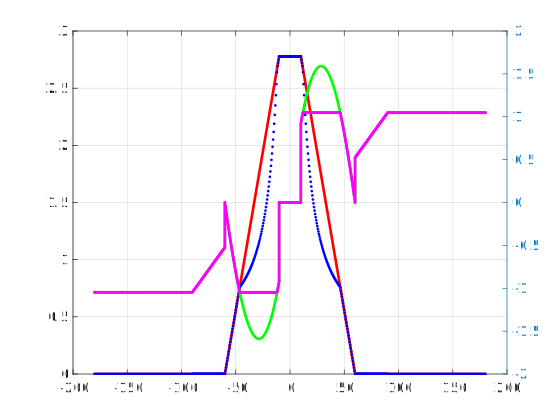
\includegraphics[scale=0.80]{Images/v_w_truncated.pdf}
    \caption{Truncated angular and linear speed.}
    \label{fig:v_w_truncated}
  \end{center}
\end{figure}
    
\end{itemize}



\section{References}

Implementation of the Pure Pursuit Path Tracking Algorithm, R. Craig Coulter, CMU-RI-TR-92-01.


\end{document}
